\chapter{Background}
    \label{chap:background}

    \section{EiT VR Village}
        \subsection{What is EiT?}
            Experts in Teamwork(EiT) is a compulsory subject for Master students at NTNU. There are about 80 villages, each with its unique village theme. The general theme for the villages are problem areas from society and working life. In each village, students are divided into groups and are to define their own project related to the village theme.\cite{EiTAbout}
            
            The point of EiT is for students to develop interdisciplinary teamwork skills. By composing each EiT village of students from a wide range of disciplines, each student will learn how to work together in interdisciplinary groups. There is also a focus on reflection of one's own contribution in a team, and reflection on the team as a whole.\cite{EiTAbout}
            
            To help the students in their reflection endeavours, EiT has employed teaching assistants to observe the students as they work. These facilitators are to help the groups by asking questions, and stating some of their observations to foster discussions and further introspection in the group. The facilitator is never to command, or directly give instructions to the group. 
        
        \subsection{VR/AR for learning and training}
            "Virtual and Augmented Reality for Learning and Training" is an EiT village led by Ekaterina Prasolova-Førland. On NTNU's page about the village it says (Translated to English): \emph{"In this village we are going to explore innovative solutions for collaboration in VR/AR with our sister-village at NTNU-Gjøvik (led by Simon McCallum). Some of the groups will therefor have the opportunity to collaborate on their projects with the Gjøvik-students in a virtual arena with HTC Vive and Hololens. The group projects can also be done in collaboration with a selection of local businesses and international actors."}
            
            This master thesis is written in collaboration with this village. It is through this village that we have gotten access to authentic users, and resources like hardware and lab space.
        
    \section{NTNU Dragvoll VR Lab}
        The VR lab at Dragvoll started out as a small repurposed office room at the department of "Education and Lifelong Learning". The space contained two computers, each connected with a HTC Vive. The Vives shared the same spatial area only divided by a digitally defined split of the room. In other words the lab was cramped and didn't support many concurrent users.
        
        In the beginning of January 2018, the lab was moved to a repurposed computer lab completely renovated to serve the purpose of a modern VR lab. At the time of writing this thesis, it contains 4 semi-separated booths, 5 VR ready computers, 4 HTC Vive setups, 3 Windows Mixed Reality headsets, one Oculus Rift, and 3 Hololenses. With all this new technology operating simultaneously in the same space, there were some unforeseen issues. These issues are addressed in section \ref{sec:vrlabfixes}.
        
    \section{Concepts}
    
        \subsection{Virtuality Continuum}
            The Virtuality Continuum(VC), as shown in Figure \ref{fig:virtualcontinuum}. \emph{"Is a concept which relates the mixture of classes of objects presented in any particular display situation."}\cite{Milgram1994} This article, "\emph{A Taxonomy of Mixed Reality Visual Displays}" by Paul Milgram and Fumio Kishino\cite{Milgram1994} introduces the concept of a "virtuality continuum" to describe the range of environments shown on any particular display. The articles focus on the taxonomy of Mixed Reality displays, and is also one of the earliest adapters of the concept of Mixed Reality.
            \begin{figure}[!ht]
                \centering
                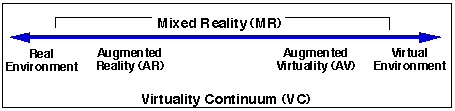
\includegraphics[scale=1]{figures/virtualcontinuum.png}
                \caption{Simplified representation of a "virtuality continuum".\cite{Milgram1994}}
                \label{fig:virtualcontinuum}
            \end{figure}
        
        \subsubsection{Virtual Reality}
            Milgram's and Kishinos's description of Virtual Reality(VR) from their paper\cite{Milgram1994}. VR is the concept of a virtual space where the user is fully immersed in a virtual world, usually through a Head Mounted Display(HMD). This means that the environment, and everything the user sees and interacts with is completely synthetic. The environment can emulate the real world and seem like reality, be it fiction or otherwise; or this Virtual Environment(VE) might be a world where our physical laws do not apply. On the virtuality continuum, as shown in Figure \ref{fig:virtualcontinuum}, this type of environment resides on the furthest extreme, opposite the real environment.
    
        \subsubsection{Augmented Reality}
            Augmented Reality(AR) is the concept of a real environment with digital elements superimposed, enhancing the users perception of reality\cite{Milgram1994}. This is achieved by rendering these digital "\emph{holograms}" on a transparent display which the user sees through(e.g. Microsoft's Hololens\cite{hololens} or Magic Leap\cite{magicleap}. The same effect can also be achieved by superimposing the digital elements onto video captured by a camera in real-time.
        
        \subsubsection{Mixed Reality}
            As shown in Figure \ref{fig:virtualcontinuum}, a Mixed Reality(MR) display can reside anywhere between the extremes of the virtuality continuum\cite{Milgram1994}. The technology has moved on since 1994, when the paper by Kishino and Milgram was published. \emph{"Since then, the application of mixed reality goes beyond displays but also includes environmental input, spatial sound, and location."}\cite{wdc-mr}
            
            Microsoft, especially, has expanded on the application of Mixed Reality. And in the article "What is mixed reality?"\cite{wdc-mr}. MR is described like this: \emph{"Most mobile phones on the market today have little to no environmental understanding capabilities. Thus the experiences they offer cannot mix between physical and digital realities. The experiences that overlay graphics on video streams of the physical world are augmented reality, and the experiences that occlude your view to present a digital experience are virtual reality. As you can see, the experiences enabled between these two extremes is mixed reality"}\cite{wdc-mr}. This spectrum is found in Figure \ref{fig:mrspectrum}
            
            \begin{figure}[!ht]
                \centering
                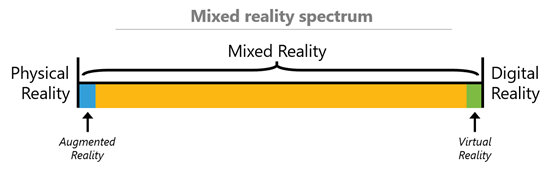
\includegraphics[scale=.85]{figures/mixedrealityspectrum.png}
                \caption{The Mixed Reality Spectrum\cite{wdc-mr}}
                \label{fig:mrspectrum}
            \end{figure}
            
            In Figure \ref{fig:mrdevicetypes} the two main device types that deliver Windows Mixed Reality is listed. These are: Holographic devices, which has the ability to place digital content in the real world\cite{wdc-mr}; and Immersive devices, which has the ability to hide the physical world and replace it with a digital experience.\cite{wdc-mr} 
            
            \begin{figure}[!ht]
                \centering
                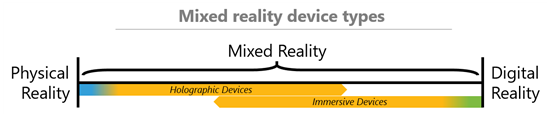
\includegraphics[scale=.85]{figures/mixedrealityspectrumdevicetypes.png}
                \caption{Mixed reality device types.\cite{wdc-mr}}
                \label{fig:mrdevicetypes}
            \end{figure}
            
        \subsection{Holograms}
            Holograms are \emph{"objects made of light and sound that appear in the world around you, just as if they were real objects."} \cite{wdc-holo} Basically they are the digital objects the user of the Hololens sees and interacts with. The objects can be placed anywhere in the room, and responds to gaze, gestures and voice commands. In our application, the hologram the user will experience, is a live version of the virtual world where the users of the immersive headsets are collaborating in. This world is scaled down to fit the table or floor.
            
        \subsection{Collaboration}
            Collaboration is by Rochelle and Teasley, defined as \emph{"a coordinated, synchronous activity that is the result of a continued attempt to construct and maintain a shared conception of a problem."}\cite{Roschelle1995}. In their paper they further distinguish 'Collaborative' problem solving and 'Cooperative' problem solving. The latter divides work between the participants, whilst the former is a mutual engagement where the participants make a coordinated effort to solve a problem together. \cite{Roschelle1995} 
            
        \subsection{Immersion} % Research and definition of what immersion means in the context of VR
            Immersion in relation to computer games is "used to describe the degree of involvement with a game" \cite{Brown2004}. In the paper by Brown in 2014 he defines three different levels of immersion: Engagement, engrossment and total immersion. Each level has its own barriers that needs to be removed for that level of immersion to be possible. Entering a higher level of immersion is correlated with having a higher level of concentration and focus \cite{Jennett2008}. For IVR-Connection this is one of the concepts that can give the user an advantage over collaborating in "real life".
        
        \subsection{Presence} % Research and definition of what presence means in the context of VR
            Jennet et al. presents two different perspectives on the definition of presence \cite{Jennett2008}. The first has basis in the rationalistic tradition, and defines presence as a psychological sense of being in a virtual environment \cite{Slater1994}. With this perspective the level of presence has to be evaluated through user feedback. The other bases itself on the Heideggerian/Gibsonian metaphysics, and relates presence to the ability of "successfully supported action in the environment" \cite{Zahorik1998}. With this perspective presence can be evaluated through empirical means. Presence and immersion have a lot in common and are often used interchangeably. However, Jennet et al. argues that presence is a state of mind, while immersion is an experience in time \cite{Jennett2008}. With this distinction presence and immersion are allowed to overlap, but it is also possible to have one without the other. For example, a user can fit the definition of being immersed while playing Tetris, but it would be hard to imagine the user feeling present in the Tetris world of falling blocks. \cite{Jennett2008}
    
    \section{Technology}
    % What technology are we using.
        In this section we will cover the technology that made everything possible. This master is based on cutting edge technology from Microsoft and Unity.
    
        \subsection{Universal Windows Platform}
        % About UWP. What is it and why we use it
            Universal Windows Platform (UWP) provides a common app platform for every device that runs Windows 10. An UWP app is written in C++ /WinRT or C++ /CX and has access to the Win32 APIs that are part of the UWP. These Win32 APIs are implemented by all Windows 10 devices.\cite{wdc-UWP} Examples of devices running Windows 10 are: Desktop computers, phones, XBOX and Hololens.
        
        \subsection{Mixed Reality Toolkit}
        % What is it and why we use it
            \emph{"The Mixed Reality Toolkit is a collection of scripts and components intended to accelerate development of applications targeting Microsoft HoloLens and Windows Mixed Reality headsets. The project is aimed at reducing barriers to entry to create mixed reality applications and contribute back to the community as we all grow."}\cite{MRToolkitReadme}
    
        \subsection{Unity}
        % What is it and why we use it
            Unity is a game engine for creating 2D, 3D, VR, AR and MR games and apps. It has its own graphics engine and a full-featured editor that enables you to create games, and deliver your content to virtually any media or device. Unity also features services like cloud building, multiplayer network, version control and analytics. Unity is also at the forefront of the growing VR market. An estimated 90\% of Samsung Gear VR games and 53\% of Oculus Rift (games at launch) were[sic] Made With Unity. \cite{UnityAbout}
        
        \subsection{Unreal}
            One of the oldest and most used game engines (20 years). Been used by multiple award winning AAA games. Written in C++ and is highly optimized for PC, VR and Mobile platforms.
            Visual coding in C++ using blueprints.
    
        \subsection{Hololens}
            The Hololens is Microsoft's holographic device. Using inside-out tracking, it is a fully mobile head mounted device running Windows 10. It has full six-degrees of freedom movement and uses a see-through display to render the "\emph{holograms}".
    
        \subsection{Immersive Headsets}
            Under the Mixed Reality Moniker, the Immersive Headsets are VR headsets that uses built-in inside-out tracking. With no need for external sensors, and only one cable for connection with the PC; One can enjoy VR from anywhere. Headsets are provided by multiple different big name retailers, all providing their own designs and solutions for the platform.
    
    \section{Related Work}
        Microsoft's MR technology is very new, for this reason there is not a lot of research and exploration on different uses of the technology. There are some collaboration oriented applications made for VR and AR platforms, VR especially has had some progress in this area. First we will introduce some technology and research that has been instrumental in the development of the Unity version of IVR-Connection.
        
        
        \subsection{The Unreal version of IVR-Connection}
            The Unreal version of IVR-Connection's main goal is to provide a Virtual Environment to facilitate collaboration. This application is a result of the master thesis \emph{Virtual Reality Collaboration: Using current virtual reality technology for long distance collaboration and meetings} by Nicklas Løkkeberg Nilsen. \cite{nilsen2017} It has since been worked on by bachelor and EiT students. It implements features for drawing on a whiteboard, image sharing, 360 video viewing, a prototype for sharing 3D models, and a prototype for simulating laser physics. Since we had to remake IVR-Connection in Unity, we still wished to provide a similar collaborative environment, albeit our thesis is focused on the facilitator spectating we originally wanted to add.
        
        \subsection{Virtual Reality Spectating}
            In the master thesis \emph{Virtual Reality Spectating}, by Jan Greger Hemb, a discussion on virtual reality spectating is conducted. Hemb builds on IVR-Connection and tries to add different forms of spectating to see which one the users prefer. His results found that virtual reality was the preferred way to spectate virtual reality, and that having freedom of movement was preferred to being limited. \cite{hemb2017}
            
        \subsection{MR Sharing 250}
            MR Sharing 250 is a tutorial from Microsoft showcasing the possibility for combining the virtual reality of immersed headsets with the augmented reality of Hololens. \cite{wdc-mr250} It contains the models and code for a small virtual environment, were the immersed headset users can solve puzzles in the environment and the Hololens users can observe them. 
            
            When developing the Unity version of IVR-Connection this tutorial was a part of the resources used. It was however not as useful as we thought it to be when we first discovered it. This tutorial and its resources had aged badly and did not support the newest updates from the Mixed Reality Toolkit and Unity. It was however possible to transfer the models and parts of the code, that with a little bit of modification gave us shortcuts to some common features. The player models were taken directly from the tutorial.
        
        \subsubsection{Augmented Reality Visualizations}
            In a recent study done by at Delft University of Technology about different ways of visualizing Augmented Reality, there was \emph{"[...] significant indications that the use of a ‘god-mode’ perspective for the remote expert provides the best situation awareness [...]"} \cite{aschenbrenner2018}. In this context 'god mode' perspective refers to observing miniaturized versions of the virtual objects. In our solution this type of perspective is used to give the facilitator a good overview over the the virtual environment.

            
        \subsection{Other uses of VR/AR/MR for collaboration}
            Listed below are some of the examples of applications for collaboration that actively uses virtual, augmented, or mixed reality as its primary medium.
            
            \subsubsection{Medical Training in Virtual Reality}
                In the master thesis \emph{Medical Procedural Training in Virtual Reality}, by Tarald Gåsbakk and Håvard Snarby, produced an application that could help train and engage medical students \cite{gaasbakk2017}. A similar application was made using Second Life in \emph{"Practicing Interprofessional Team Communication and Collaboration in a Smart Virtual University Hospital"} \cite{Prasolova-Forland2018}

            \subsubsection{Masters of Pi}
                Master of Pi is a project that aims to redefine Product Lifecycle Management software by using VR technology. They want to do this by providing a collaborative, interactive digital space in which engineers can work across disciplines. This can reduce cost and complexity associated with constant refactoring of CAD data. \cite{mastersofpi}
            
            \subsubsection{CocoVerse}    
                CocoVerse\cite{Greenwald2017} is an application quite similar to the original IVR-Connection, both have the same idea of providing a virtual environment for collaboration. CocoVerse provides a way for users to \emph{"[...] sketch volumetric surfaces in 3D with a
                virtual paintbrush; create and manipulate objects; capture images with a camera, and place them as pictures; and
                write phrases using a speech-to-text system."}
            
            \subsubsection{check jabref}
    \section{Theory}
        \chapter{Theory}

    \section{Collaboration}
    
        \subsection{Collaboration supported by technology}
    
        \subsection{Collocated Collaboration}
        
        \subsection{Remote Collaboration}
    
    \section{Collaborative Learning}
        Collaborative learning is, according to Dillenbourg, \emph{"a situation in which particular forms of interaction among people are expected to occur, which would trigger learning mechanisms".} \cite{dillenbourg1999} This definition, though it is very broad, helps expose the critical element of learning collaboratively. Namely triggering the learning mechanisms. Dillenbourg proposes four categories of ways to increase the probability of triggering these mechanisms: Setting up the initial condition, over-specify the 'collaboration' contract with a scenario based on roles, scaffold productive interactions by encompassing interaction rules in the medium, and monitor and regulate the interactions.
        
        A similar and more clearly defined division was proposed by a paper by Lee, with some additions and modifications. It divides collaborative learning into six procedural elements meant to distinguish collaborative learning from other types of small-group learning: Intentional group formation, continuity of group interaction, interdependence between group members, individual accountability, explicit attention to the development of social skills, and instructor as facilitator. \cite{Lee2009}
        
        Intentional group formation entails designing the group based on learning goals and activities, which lines up with Dillenbourg's category of setting up the initial condition. Continuity of group interaction adds a requirement for the group to sustain their discussion and interactions over a substantial or extended period of time. Interdependence between group members entails creating a perception for group members that they are linked in a way that one cannot succeed unless everyone succeeds, which lines up with Dillenbourg's category of over-specify the 'collaboration' contract with a scenario based on roles. Individual accountability adds that the group members need to be accountable for their own performance as well as that of the group. Explicit attention to the development of social skills entails taking deliberate steps to foster social competencies, which lines up with Dillenbourg's category of scaffold productive interactions by encompassing interaction rules in the medium. Instructor as facilitator dictates that the instructor should take the role of a facilitator, which lines up with Dillenbourg's category of monitoring and regulating the interactions.
        
        This indicates that by supporting the six procedural elements proposed by Lee, can be a way to trigger the learning mechanisms that can be accessed by working collaboratively.

        \subsection{Project Based Learning}
        This is how EiT Works
        
        \subsection{Computer Supported Collaborative Learning}
    
    \section{Facilitation}
        \subsection{Facilitating for CSCL}
        This is what we want to do